% !TEX root =  master.tex
\chapter{Analyse} \label{analyse}
	
	Analyse für den Durchblick.
	Studium, Modul \enquote{Fallstudie} et cetera
	
	\section{Anforderungsanalyse}
	
	\section{Ist-Analyse}
	Bestandsaufnahme existierender Reservierungssysteme
	
	\section{Soll-Analyse}
		
	 	\subsection{User-Research-Prozess} 
	 	User Research ist eine systematische Untersuchung der Ziele, Bedürfnisse und Fähigkeiten der Benutzer\autocite[Vgl.][S. 6]{Schumacher.2010}.
	 	Durch diesen Prozess lässt sich sicherstellen, dass die entwickelte Software den Nutzern einen Mehrwert bietet und an deren Bedürfnisse angepasst ist.
		Der Prozess startet mit der Definition der \textit{User Profile}. Diese klassifizieren Endanwender mit Nutzerprofilen, damit eine konkrete Vorstellung der Anwender geschaffen wird. Anhand von detaillierten Beschreibungen von Attributen lässt sich die Nutzergruppe identifizieren.
		
		\begin{table}[H]
			\centering
			\begin{tabular}{p{5,5cm} || c | c }
				\textbf{Attribute} & \textbf{Endanwender} & \textbf{Mitarbeiter} \\\toprule
				Alter &  16 - 99 Jahre &  16 - 99 Jahre \\
				Geschlecht &  männlich und weiblich &  männlich und weiblich  \\
				Medienkompetenz &  ja und nein &  ja  \\
				Erfahrung Onlinereservierung &  ja und nein &  ja  \\
			\end{tabular}
			\caption[User Profile]{\label{tab:tabelleUserProfile}User Profile}
		\end{table}
		
		Im nächsten Schritt werden Personas aus den User Profiles erstellt. Personas sind fiktive Personen, die für eine Nutzergruppe steht. Der Zweck von Personas ist, dass Entwickler Empathie und Einfühlungsvermögen zu den konkreten Anwendern aufbauen können. 
		
		\begin{figure}[H]
			\subfigure[Persona Franzi]{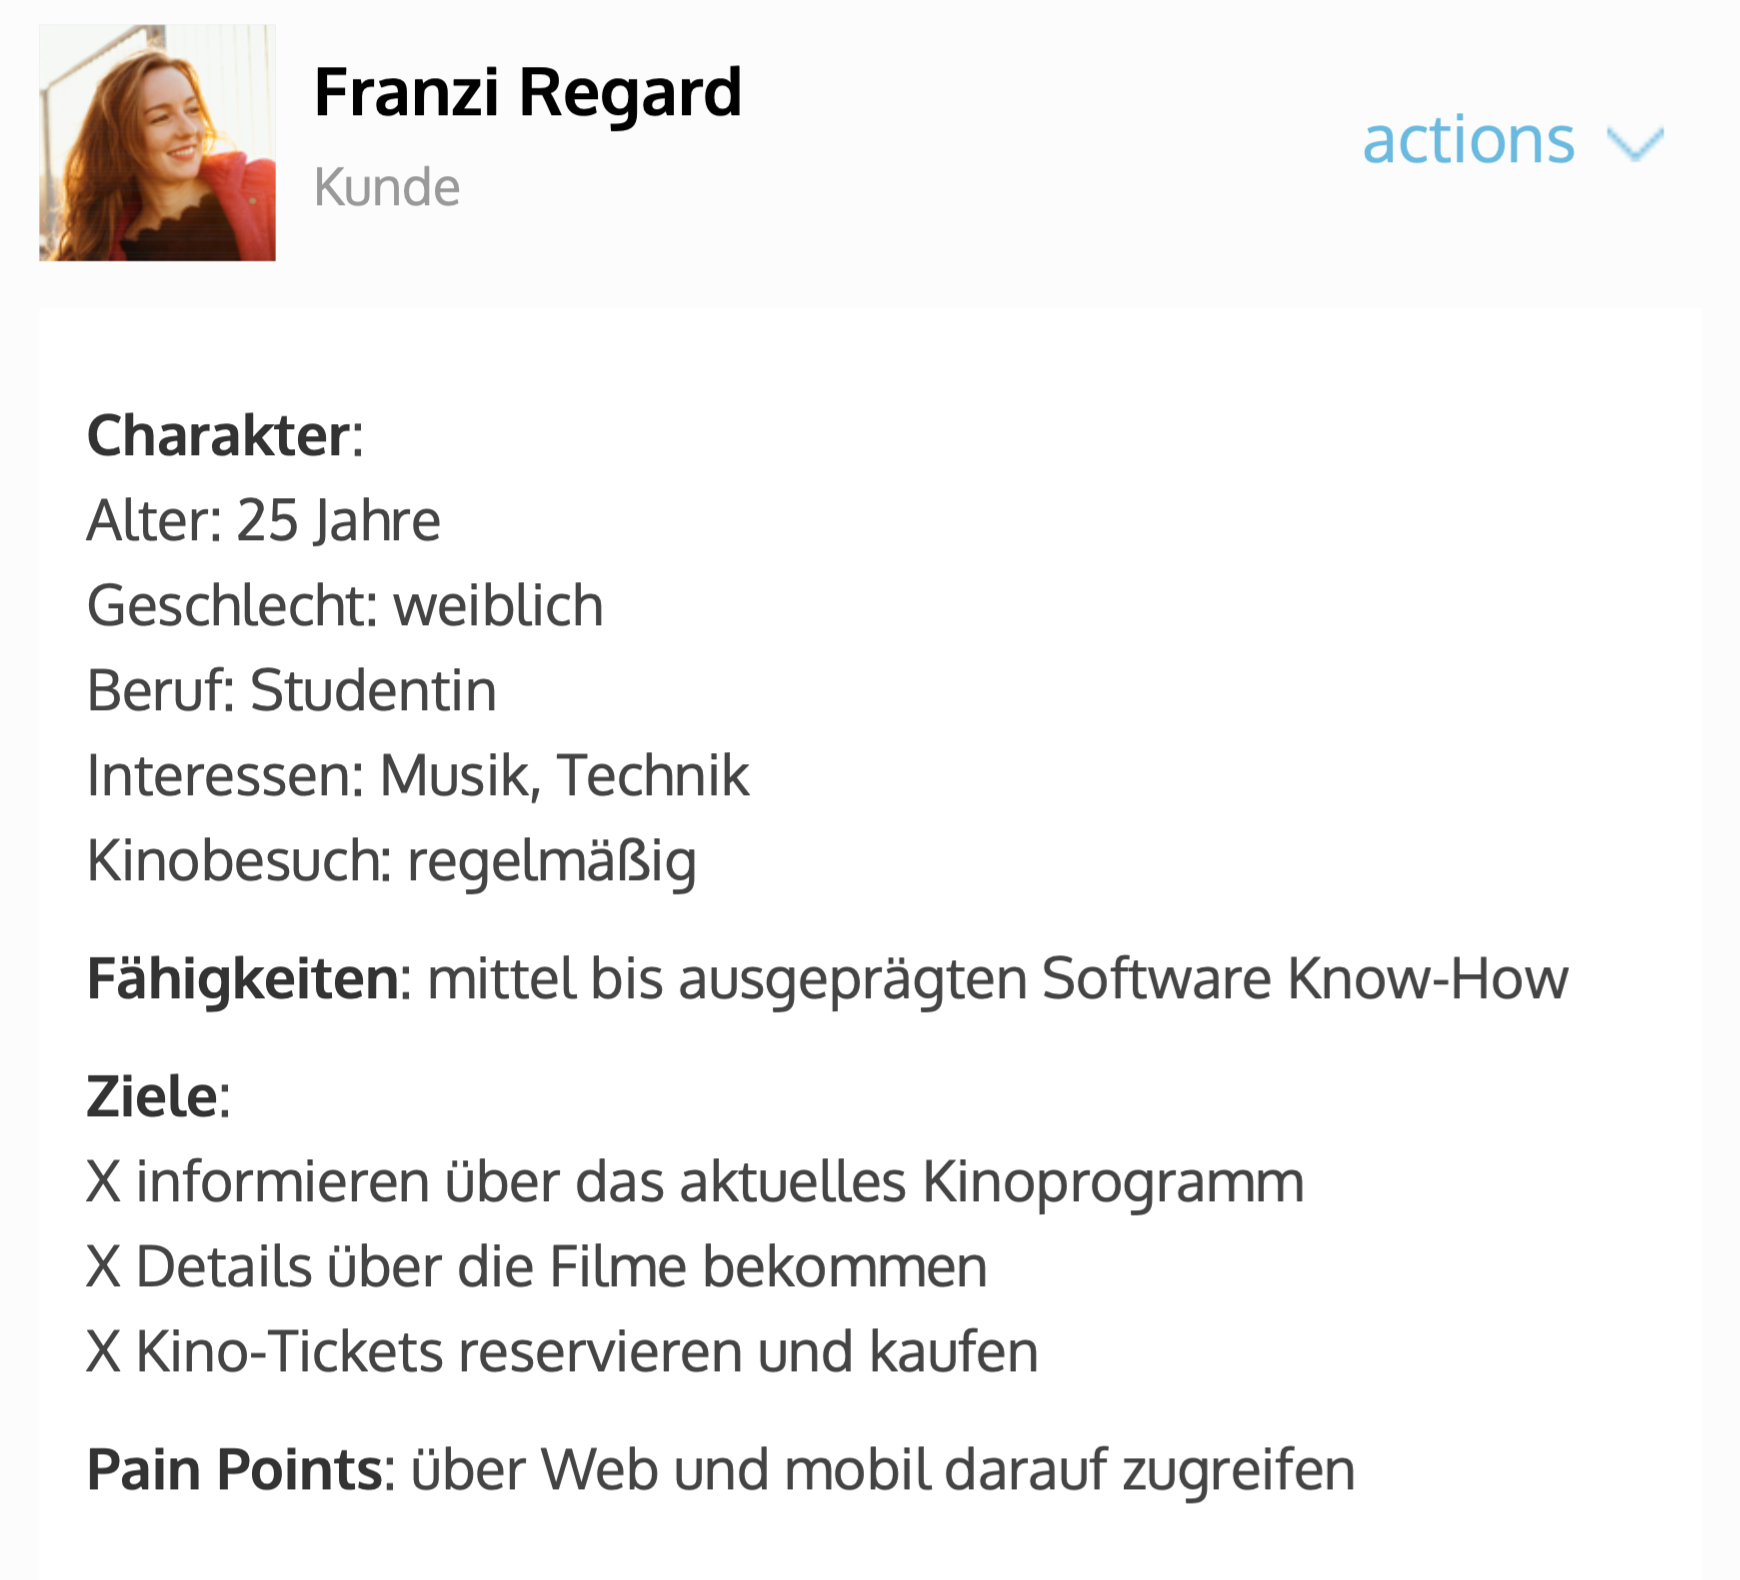
\includegraphics[width=0.49\textwidth]{img/franzi.png}} 
			\subfigure[Persona Gustav]{
\includegraphics[width=0.49\textwidth]{img/gustav.png}} 
			\subfigure[Persona Kassandra]{
\includegraphics[width=0.49\textwidth]{img/kassandra.png}} 
			\subfigure[Persona Walter]{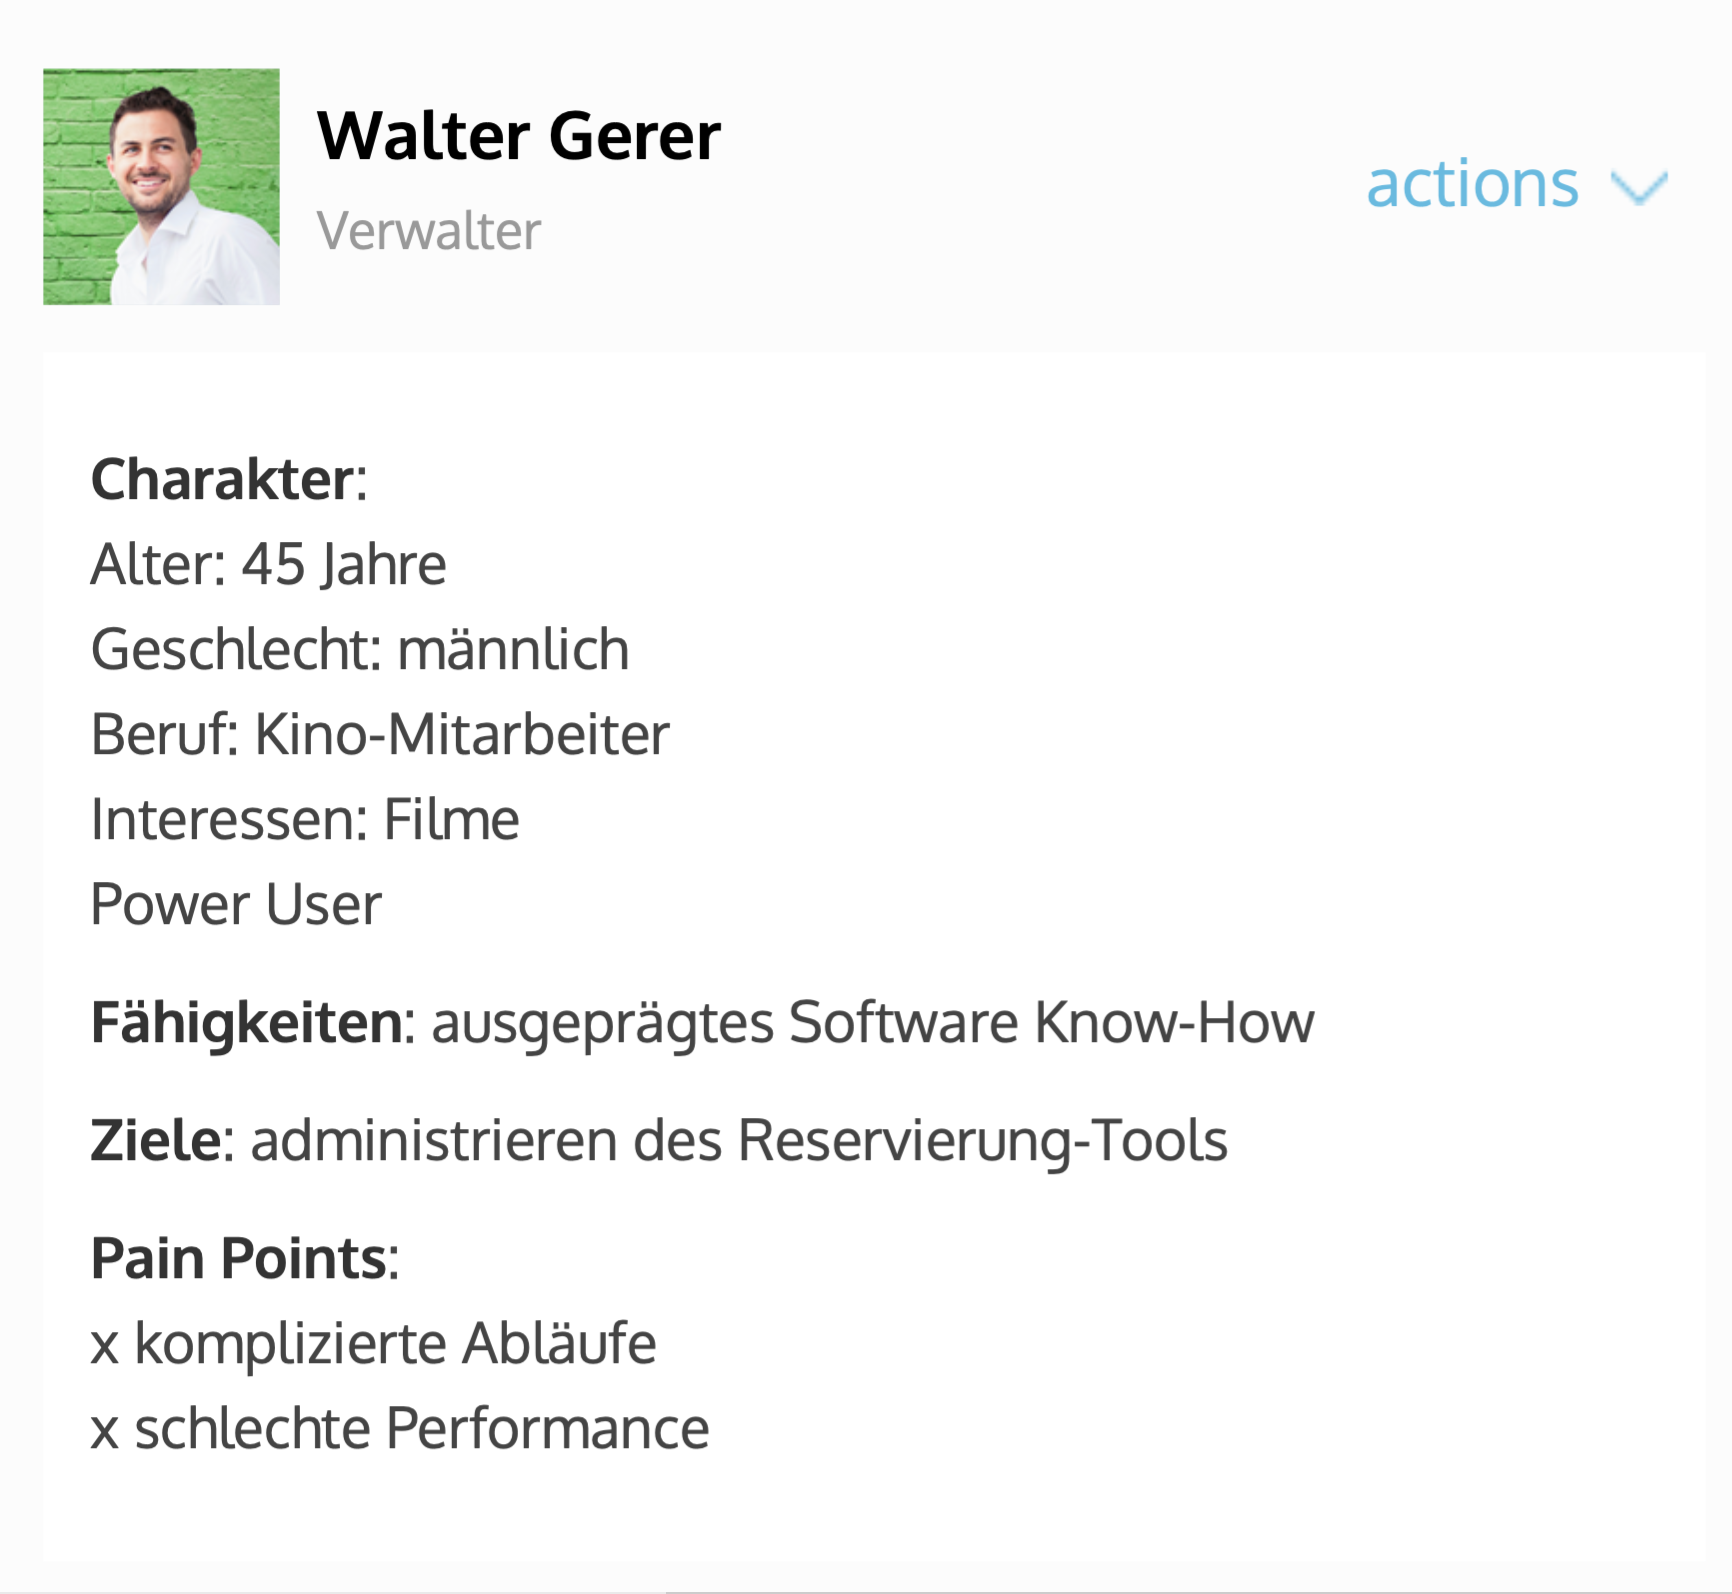
\includegraphics[width=0.49\textwidth]{img/walter.png}} 
			\caption[Personas ]{\label{fig:personas}Personas [DRAFT - detaillierter!] }
		\end{figure} 
		
		Darauf aufbauend werden Use Cases für die Personas entwickelt. Diese beschreiben Szenarien, wie die Personas das Endprodukt verwenden werden und welche Vorgehensweisen und Anforderungen dabei haben. 
		
		\begin{figure}[H]
			\begin{tabular}{p{13cm}}
				\textbf{Franzi Regard} \\\toprule
				Als Franzi möchte ich mich schnell vom meinem Smartphone oder Laptop aus über das aktuelle Kino-Programm informieren und Kino-Tickets reservieren und kaufen, um mit meinen Freunden einen Film anzuschauen. Dabei lege ich viel Wert auf ansprechendes Design und eine schnelle Abwicklung.
			\end{tabular}
			\caption[Use Case Franzi]{\label{fig:useCaseFranzi} Use Case Franzi [DRAFT]}
		\end{figure}
	
		\begin{figure}[H]
			\begin{tabular}{p{13cm}}
				\textbf{Gustav Gast} \\\toprule
				Als Gustav möchte ich Kino-Tickets reservieren, um mit meiner Familie einen Familienabend zu verbringen. Eine intuitive Anwendung ist für mich sehr wichtig, weil noch nie online Tickets reserviert habe. 
			\end{tabular}
			\caption[Use Case Gustav]{\label{fig:useCaseGustav} Use Case Gustav [DRAFT]}
		\end{figure}
	
		\begin{figure}[H]
			\begin{tabular}{p{13cm}}
				\textbf{Kassandra Caisse} \\\toprule
				Als Kassandra möchte ich mir die Reservierungen anschauen und Reservierungen anpassen können. 
			\end{tabular}
			\caption[Use Case Kassandra]{\label{fig:useCaseKassandra} Use Case Kassandra [DRAFT]}
		\end{figure}

		\begin{figure}[H]
			\begin{tabular}{p{13cm}}
				\textbf{Walter Gerer} \\\toprule
				Als Walter möchte ich das Kino-Programm verwalten und einpflegen. 
			\end{tabular}
			\caption[Use Case Walter]{\label{fig:useCaseWalter} Use Case Walter [DRAFT]}
		\end{figure}
		
		Schließlich wird aus den Personas eine User-Story-Map erstellt. In dieser werden die daraus hervorgehenden Features visuell geplant und in unterschiedliche Releases priorisiert. 
		
	\begin{center}
		{\textbf{[User-Story-Map // Größe?]}}
	\end{center}
		
	 	
%		\subsection{Vorgabe}
%		\subsection{Rahmenbedingungen}
%		\subsection{Bewertungskriterien}